% Unofficial University of Cambridge Poster Template
% https://github.com/andiac/gemini-cam
% a fork of https://github.com/anishathalye/gemini
% also refer to https://github.com/k4rtik/uchicago-poster

\documentclass[final]{beamer}

% ====================
% Packages
% ====================

\usepackage[T1]{fontenc}
\usepackage{lmodern}
\usepackage[orientation=portrait,size=custom,width=100,height=120,scale=1.0]{beamerposter}
\usetheme{gemini}
\usecolortheme{nott}
\usepackage{graphicx}
\usepackage{booktabs}
\usepackage{subcaption}
\usepackage{multicol}
\usepackage{tikz}
\usepackage{pgfplots}
\pgfplotsset{compat=1.14}
\usepackage{anyfontsize}
\usepackage{xcolor}
\renewcommand{\normalsize}{\fontsize{36}{40}\selectfont} % Aumenta de ~24pt a ~28pt

% ====================
% Lengths
% ====================

% If you have N columns, choose \sepwidth and \colwidth such that
% (N+1)*\sepwidth + N*\colwidth = \paperwidth
\newlength{\sepwidth}
\newlength{\colwidth}
\setlength{\sepwidth}{0.025\paperwidth}
\setlength{\colwidth}{0.45\paperwidth}

\newcommand{\separatorcolumn}{\begin{column}{\sepwidth}\end{column}}

  % ====================
  % Title
  % ====================

  \title{Transmisión de ondas electromagnéticas en estructuras de Moiré para dieléctricos.}

  \author{Sergio Montoya Ramírez \and Juan Gabriel Ramirez Rojas \and Daniel Rueda Villalba\inst{1}}

  \institute[shortinst]{\inst{1} Universidad de los Andes}

  % ====================
  % Footer (optional)
  % ====================

  % \footercontent{
  %   \href{https://utfpr.edu.br/ct/ppgca}{utfpr.edu.br/ct/ppgca} \hfill
  %   Mostra de Trabalhos do PPGCA --- TechTalks 2024 \hfill
  %   \href{mailto:ppgca-ct@utfpr.edu.br}{ppgca-ct@utfpr.edu.br}}
  % (can be left out to remove footer)

  % ====================
  % Logo (optional)
  % ====================

  % use this to include logos on the left and/or right side of the header:
  \logoright{
\includegraphics[height=5cm]{./logos/logo-uniandes.png}}
  %\logoleft{\hspace{20ex}
\includegraphics[height=3.5cm]{logos/ppgca-logo.png}}

  % ====================
  % Body
  % ====================

  \begin{document}

  \begin{frame}[t]
    \begin{columns}[t]
      \separatorcolumn

      \begin{column}{\colwidth}

        \begin{block}{Introducción}
          Los cristales fotónicos son estructuras con un índice de refracción periódico que dan lugar a complejas estructuras de bandas. Un caso de particular interés físico surge al rotar dos de estas capas entre sí. Esto genera patrones de Moiré que incrementan considerablemente el tamaño de la celda unitaria del cristal, alterando drásticamente sus propiedades y su estructura de bandas.

          Sin embargo, los métodos convencionales para simular estos sistemas se basan en discretizar el espacio y resolver cada capa de manera independiente mediante álgebra lineal. El aumento de tamaño y complejidad de las celdas unitarias representa un reto computacional prohibitivo. Este trabajo se centra en el estudio, simulación y comprobación experimental de cristales dieléctricos con patrones de Moiré utilizando el método \textit{RCWA-4D}.
        \end{block}


        \begin{block}{Objetivos}
          \begin{itemize}
            \item Estudiar el método \textit{RCWA-4D} para simular la transmisión en cristales fotónicos dieléctricos con patrones de Moiré en función de su ángulo de rotación.
            \item Simular diversas estructuras computacionales para identificar configuraciones de interés en materiales de fácil acceso.
            \item Reproducir experimentalmente los diseños analizados para validar la precisión y exactitud del modelo teórico.
          \end{itemize}
        \end{block}

        \begin{block}{Patrones de Moiré}
          Un patrón de Moiré surge de la superposición y rotación relativa de dos redes periódicas. En el espacio recíproco, la rotación implica que los nuevos vectores de la red de Moiré ($\mathbf{G}_M$) se construyen a partir de la interferencia de los vectores de las capas individuales \cite{lou2025rcwa4d}:

          \begin{equation}
          \mathbf{G}_M = \mathbf{G}_1 - \mathbf{G}_2
          \end{equation}

          Como se ilustra a continuación, esta interferencia geométrica genera nuevas periodicidades a mayor escala, lo que modifica sustancialmente las características físicas del material.

          \begin{figure}[h]
            \centering
            \begin{minipage}[t]{0.45\linewidth}
              \centering
              \begin{tikzpicture}[scale=1.2]
                \def\lado{15}
                \def\espaciado{0.1}
                \def\angulo{0}
                \colorlet{redLayer}{red!60!black!50}
                \colorlet{blueLayer}{cyan!70!black!60}
                \begin{scope}[redLayer]
                  \foreach \i in {0,\espaciado,...,\lado} {
                    \draw[very thin] (\i,0) -- (\i,\lado);
                    \draw[very thin] (0,\i) -- (\lado,\i);
                  }
                \end{scope}
                \begin{scope}[blueLayer, rotate around={\angulo:(\lado/2, \lado/2)}]
                  \foreach \i in {0,\espaciado,...,\lado} {
                    \draw[very thin] (\i,0) -- (\i,\lado);
                    \draw[very thin] (0,\i) -- (\lado,\i);
                  }
                \end{scope}
                \node[anchor=north west, font=\sffamily\small] at (0,0) {$\theta = \angulo^\circ$};
              \end{tikzpicture}
              \subcaption{Ángulo de rotación $0^\circ$}\label{fig:moire0}
            \end{minipage}\hfill
            \begin{minipage}[t]{0.45\linewidth}
              \centering
              \begin{tikzpicture}[scale=1.2]
                \def\lado{15}
                \def\espaciado{0.1}
                \def\angulo{5}
                \colorlet{redLayer}{red!60!black!50}
                \colorlet{blueLayer}{cyan!70!black!60}
                \begin{scope}[redLayer]
                  \foreach \i in {0,\espaciado,...,\lado} {
                    \draw[very thin] (\i,0) -- (\i,\lado);
                    \draw[very thin] (0,\i) -- (\lado,\i);
                  }
                \end{scope}
                \begin{scope}[blueLayer, rotate around={\angulo:(\lado/2, \lado/2)}]
                  \foreach \i in {0,\espaciado,...,\lado} {
                    \draw[very thin] (\i,0) -- (\i,\lado);
                    \draw[very thin] (0,\i) -- (\lado,\i);
                  }
                \end{scope}
                \node[anchor=north west, font=\sffamily\small] at (0,0) {$\theta = \angulo^\circ$};
              \end{tikzpicture}
              \subcaption{Ángulo de rotación $5^\circ$}\label{fig:moire5}
            \end{minipage}
            \caption{Patrones de Moiré generados al rotar una rejilla cuadrada sobre otra.}
            \label{fig:moire}
          \end{figure}
        \end{block}

        \begin{block}{RCWA-4D}
          El Análisis Riguroso de Ondas Acopladas (\textit{RCWA}) simula estructuras aproximándolas a capas discretas. Resuelve las ecuaciones de Maxwell expandiendo los campos electromagnéticos en ondas planas:

          \begin{equation}
            \mathbf{E}(\mathbf{r}) = \sum_{\mathbf{G}} \mathbf{E}_{\mathbf{G}}(z) e^{-i(\mathbf{k} + \mathbf{G})\cdot \mathbf{r}_\parallel}
          \end{equation}

          Al ser discreto, las propiedades de transmisión y reflexión se formulan matricialmente (\textit{S-matrices}). Las capas se conectan igualando sus condiciones de frontera mediante el producto estrella de Redheffer ($\otimes$) \cite{lou2025rcwa4d}.

          % SUGERENCIA: Aquí puedes insertar una pequeña figura o diagrama en TikZ que muestre S_1 \otimes S_2 si tienes espacio.

          No obstante, la expansión de la celda unitaria en los patrones de Moiré hace que el \textit{RCWA} tradicional sea inmanejable. El modelo \textit{RCWA-4D} soluciona esto proyectando la segunda capa en función de la primera, construyendo un espacio recíproco extendido que depende de ambas periodicidades ($\mathbf{G}_1$ y $\mathbf{G}_2$). Esto reduce computacionalmente el problema: se pasa de resolver dos matrices bidimensionales sumamente densas, a diagonalizar una única matriz semicuatridimensional dispersa, viabilizando la simulación.
        \end{block}


      \end{column}
      \separatorcolumn

      \begin{column}{\colwidth}

        \begin{block}{Condiciones de Simulación}
          \begin{itemize}
            \item \textbf{Propiedades ópticas:} Los índices de refracción se obtuvieron de \textit{The Materials Project}. Para el PMMA, se usaron parámetros empíricos de la literatura \cite{Tanwar2006}.
            \item \textbf{Geometría:} Se simularon dos arreglos fundamentales viables para manufactura:
          \end{itemize}

          \vspace{0.3em}
          \begin{center}
            \begin{tikzpicture}[scale=12] 
              \draw[step=1cm,gray!20,very thin] (-0.5,-0.5) grid (0.5,0.5);
              \draw[thick] (-0.5,-0.5) rectangle (0.5,0.5);
              \fill[blue!70!black, opacity=0.8] (0,0) circle (0.25);
              \node at (0,-0.7) {\footnotesize \textbf{Arreglo de orificios} ($r=0.25$)};
            \end{tikzpicture}
            \hspace{1.5cm}
            \begin{tikzpicture}[scale=12]
              \draw[step=1cm,gray!20,very thin] (-0.5,-0.5) grid (0.5,0.5);
              \draw[thick] (-0.5,-0.5) rectangle (0.5,0.5);
              \fill[red!70!black, opacity=0.8] (-0.5, -0.25) rectangle (0.5, 0.25);
              \node at (0,-0.7) {\footnotesize \textbf{Arreglo de franjas} ($|y| \leq r$)};
            \end{tikzpicture}
          \end{center}
        \end{block}

        \begin{block}{Resultados Computacionales}
          Tras simular la transmisión en más de 80 materiales, se seleccionó el \textit{PMMA} (acrílico comercial). Este dieléctrico ofrece el balance ideal entre firmas de transmisión distinguibles de Moiré y viabilidad física para su mecanizado.

          \vspace{0.3em}
          \begin{center}
            \begin{minipage}{0.48\textwidth}
              \centering
              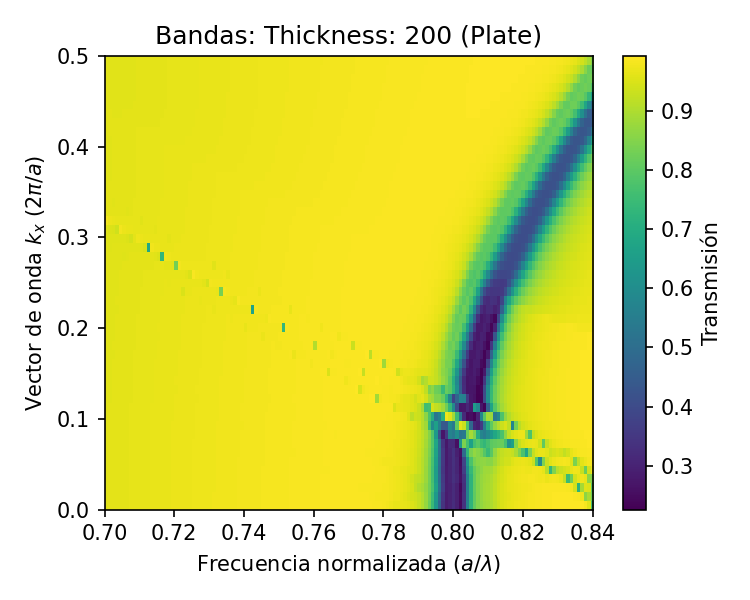
\includegraphics[width=\textwidth]{./imgs/plate.png}
              \captionof{figure}{Patrón de orificios en PMMA ($0.2 \text{ mm}$).}
              \label{fig:plate}
            \end{minipage}\hfill
            \begin{minipage}{0.48\textwidth}
              \centering
              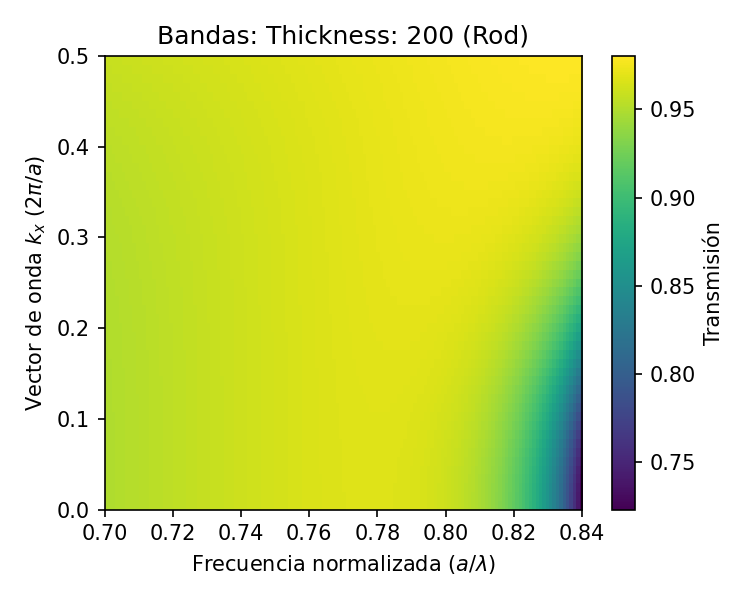
\includegraphics[width=\textwidth]{./imgs/rod.png}
              \captionof{figure}{Patrón de franjas en PMMA ($0.2 \text{ mm}$).}
              \label{fig:rod}
            \end{minipage}
          \end{center}
        \end{block}

        \begin{block}{Metodología Experimental y CAD}
          Para garantizar la fidelidad teórica-experimental, se desarrolló un programa de automatización fundamentado en el espacio real. Desde una única parametrización geométrica, el código genera simultáneamente las matrices de \textit{NumPy} para la simulación numérica y los archivos CAD vectoriales para la cortadora láser. 

          Este flujo de trabajo elimina las discrepancias morfológicas. Actualmente, el proyecto está en fase de manufactura: las estructuras de PMMA se encuentran en mecanizado para su posterior caracterización óptica.
        \end{block}

        \begin{block}{Conclusiones Preliminares}
          \begin{itemize}
            \item El método \textit{RCWA-4D} es computacionalmente eficiente para modelar superredes de Moiré, evadiendo la explosión dimensional de algoritmos convencionales.
            \item El análisis masivo demostró que el PMMA es un medio dieléctrico excelente para replicar físicamente estas estructuras periódicas rotadas.
            \item La generación simultánea del modelo numérico y el diseño físico establece una metodología robusta y libre de error humano en el ciclo de diseño.
          \end{itemize}
        \end{block}

        \begin{block}{Referencias}
          \nocite{*}
          \footnotesize
          \begin{multicols}{2}
            \bibliographystyle{plain}
            \bibliography{poster}
          \end{multicols}
        \end{block}
      \end{column}
      \separatorcolumn


    \end{columns}
  \end{frame}

\end{document}
